%--------------------------------------------------------------------------------------------------------------------
%------------------------------------------------- Chapter 9 --------------------------------------------------------
\chapter{Otras implementaciones de los ContratosDHD} \label{implementaciones}
%\pagenumbering{arabic}

\section{Condicionales DEVS en la coordinación de contratos sensibles al
contexto para los DHD}

\subsection{Introducción}

El actual contexto físico-virtual que se construye a partir de la utilización de
las Tecnologías de la Información y Comunicación (TIC) posibilita a los sujetos
ser partícipes de redes sociotécnicas conformadas por una multiplicidad de
componentes y relaciones, que se configuran y reconfiguran por las diversas
interacciones en función de una gran diversidad de requerimientos. En este
sentido, el Programa interdisciplinario de I+D+T “Dispositivos Hipermediales
Dinámicos” (DHD) [1], radicado en CIFASIS (CONICET-UNR-UPCAM), estudia la
complejidad evidente de las mencionadas redes, integrando aportes de diversas
disciplinas como informática, educación, ingeniería, psicología y antropología,
entre otras.


Se conceptualiza como Dispositivo Hipermedial Dinámico -DHD- a la red
heterogénea [2] conformada por la conjunción de tecnologías y aspectos sociales
que posibilitan a los sujetos realizar acciones en interacción responsable con
el otro para investigar, aprender, dialogar, confrontar, componer, evaluar, bajo
la modalidad de taller físico-virtual, utilizando la potencialidad
comunicacional, transformadora y abierta de lo hipermedial, regulados según el
caso, por una “coordinación de contratos” [3].
En la implementación y optimización de un DHD para la producción y diseminación
de conocimiento, los mecanismos de medición y evaluación suponen una de las
actividades principales para el análisis y el aseguramiento de la calidad de lo
que se desarrolla a través de los mismos.

Los procesos de medición son fundamentales dado que permiten cuantificar un
conjunto de características deseadas acerca de un aspecto específico de algún
ente en particular, proveyendo una visión más o menos detallada de su estado o
condición. Por su parte, la evaluación interpreta los valores obtenidos en la
medición. Para dichos procesos de medición y evaluación es necesario obtener
datos cuantitativos, a partir de métricas de atributos de entes y la posterior
interpretación de la medida a partir de indicadores [4].
Funcionalmente el DHD es conceptualizado como sistema complejo [5], en el cual
los Participantes (P) a través del intercambio analítico y de producción de
textos mediatizados en diversos tipos de formatos digitales, construyen las
posibilidades y limitaciones de la mediación interdisciplinaria responsable en
su área de incumbencia, siendo deseable que se pueda observar un paulatino
cambio en su situación contextual. Al constatar que la característica primordial
del DHD, es que las interacciones se deben a la ocurrencia asincrónica de
eventos, hemos optado por el modelado con DEVS, Discrete Event System
specification [6], considerándose además la gran adaptación del formalismo para
modelizar sistemas complejos, y su simplicidad y eficiencia en la implementación
de simulaciones.


Tecnológicamente el DHD está provista por un agregado de una pieza de software
para la inyección de propiedades de coordinación de contratos sensibles al
contexto [7]. Esta propiedad se logra a través de la implementación de contratos
[8] con mencanizmos de coordinación y componentes de sistemas context aware [9].
La utilización de reglas es parte esencial en la implementación de las acciones
de los contratos y las tareas de coordinación. A su vez, las reglas están
compuestas por los condicionales donde se centra parte de la lógica de
adaptación que se requiere en los DHD. Algunos condicionales implementados
requieren de mecanismos externos que colaboren en la composición de sus valores
de verdad [10].

En este trabajo se define un nuevo tipo de condicional, denominado Condicional
DEVS, para la inclusión de valores de verdad que puedan ser inferidos por medio
de la implementación de un conjunto de métricas flexibles que contemplan las
principales características de las interacciones de los participantes de los
DHD. Tras esta introducción, en la sección 2 se identifican los elementos de los
DHD en relación directa con los Condicionales DEVS. Luego, en la sección 3 se
presenta un modelo de integración para el funcionamiento en una herramienta del
framework SAKAI (para la justificación de dicha elección ver [7]). En la sección
4 se describen algunas de las características principales de las métricas y un
caso de uso concreto. Para finalizar, se presentan las conclusiones y
consideraciones generales.

\subsection{Aspecto tecnológico de los DHD}

En esta sección se describen aspectos tecnológicos y componentes de los DHD que
intervienen en el modelo de integración entre las métricas DEVS y el framework
de nuestra propuesta. De esta manera, se solucionan los requerimientos sobre
adaptación dinámica mediante la construcción de un modelo de contrato orientado
a la implementación de servicios sensibles al contexto.

El uso de contratos parte de la noción de Programación por Contrato
(”Programming by Contract”) de Meyer [8] basada en la metáfora de que un
elemento de un sistema de software colabora con otro, manteniendo obligaciones y
beneficios mutuos. En nuestro dominio de aplicación consideraremos que un objeto
cliente y un objeto servidor “acuerdan” a través de un contrato, -representado
con un nuevo objeto-, que el objeto servidor satisfaga el pedido del cliente, y
al mismo tiempo el cliente cumpla con las condiciones impuestas por el
proveedor. A su vez las decisiones de comportamiento partirán de los
condicionales de las acciones de los contratos.


Como ejemplo de la aplicación de la idea de Meyer en nuestro dominio de sistemas
e-learning planteamos la situación en que un usuario (cliente) utiliza un
servicio de edición de mensajes (servidor) a través de un contrato que
garantizará las siguientes condiciones: el usuario debe poder editar aquellos
mensajes que tiene autorización según su perfil (obligación del proveedor y
beneficio del cliente); el proveedor debe tener acceso a la información del
perfil del usuario (obligación del cliente y beneficio del proveedor).
A partir de la conceptualización de contratos según Meyer se propone una
extensión por medio del agregado de nuevas componentes para instrumentar
mecanismos que permitan ejecutar acciones dependiendo del contexto. En
aplicaciones sensibles al contexto [9], el contexto (o información de contexto)
es definido como la información que puede ser usada para caracterizar la
situación de una entidad más allá de los atributos que la definen. En nuestro
caso, una entidad es un usuario (alumno, docente, etc.), lugar (aula,
biblioteca, sala de consulta, etc.), recurso (impresora, fax, etc.), u objeto
(examen, trabajo práctico, etc.) que se comunica con otra entidad a través del
contrato.


En [2] se propone una especificación del concepto de contexto partiendo de las
consideraciones de Dourish [11] y adaptadas al dominio e-learning, que será la
que consideraremos en este trabajo. Contexto es todo tipo de información que
pueda ser censada y procesada, a través de la aplicación e-learning, que
caracterizan a un usuario o entorno, por ejemplo: intervenciones en los foros,
promedios de notas, habilidades, niveles de conocimientos, máquinas (direcciones
ip) conectadas, nivel de intervención en los foros, cantidad de usuarios
conectados, fechas y horarios, estadísticas sobre cursos, etc.

En términos generales, la coordinación de contratos es una conexión establecida
entre un grupo de objetos influidas por condicionales que representan parte de
la lógica de adaptación, aunque en este trabajo se consideran sólo dos objetos:
un cliente y un servidor. Cuando un objeto cliente efectúa una llamada a un
objeto servidor (ej., el servicio de edición de la herramienta Foro), el
contrato “intercepta” la llamada y establece una nueva relación teniendo en
cuenta el contexto del objeto cliente, el del objeto servidor, e información
relevante adquirida y representada como contexto del entorno [1]. En este
trabajo en los condicionales de las reglas se representarán diferente tipo de
información de contexto con distinto grado de representación y abstracción,
donde se requieren mecanismos de inferencias basados en la recolección,
representación y simulación.

A continuación se brindarán detalles sobre algunas de los componentes y
relaciones esenciales para la integración de este modelo con el framework
utilizado y con los módulos que instrumentan la coordinación de contratos.


\begin{center}
 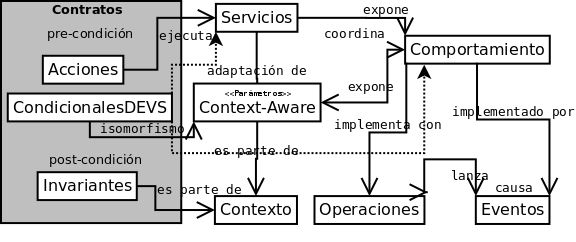
\includegraphics[width=5 in,totalheight=4 in] {Ch9/f1}
 % .: 0x0 pixel, 0dpi, 0.00x0.00 cm, bb=
\end{center}
\caption{Modelo de elementos y relaciones de los DEVS condicionales.}


Un contrato que siga las ideas de Meyer contiene toda la información sobre los
servicios que utilizarán los clientes. Para incorporar sensibilidad al contexto
nuestros contratos deberán tener referencias sobre algún tipo de información de
contexto para su utilización. En el diagrama de relaciones entre entidades
mostrado en la Figura 1 se describen los elementos que componen el concepto de
contrato sensible al contexto donde se tiene participación de los condicionales
DEVS. La figura comienza con la representación de un contrato según Meyer donde
se caracterizan los principales elementos que lo componen (pre-condiciones,
acciones, pos-condiciones). La flechas salientes de la zona gris indican los dos
tipos de relaciones (acción-servicio e invariante-contexto) que se debe
instrumentar para incorporar un mecanismo que provea a los contratos de la
característica de sensibilidad al contexto. En la porción derecha de la Figura 1
aparecen las entidades necesarias para obtener contratos sensibles al contexto.

A continuación se explica cada uno de los elementos y su relación con los
condicionales de las acciones.

- \textbf{Servicios}: En esta componente se representan los elementos necesarios
para la identificación y clasificación de los servicios que pueden formar parte
de las acciones de los contratos. Por ejemplo, nombre del servicio,
identificadores, alcance, propósito, etc. En este caso existe una relación
indirecta con el condicional DEVS establecida por la relación ejecutar entre la
acción del contrato y el servicio. 

- \textbf{Comportamiento}: El comportamiento de un servicio se logra a partir de
combinar operaciones y eventos que son representadas con las componentes
Operaciones y Eventos. De la misma manera el servicio puede ser implementado a
través del uso de eventos, representados con el componente Eventos, que puede
lanzar operaciones del componente Operaciones. Por ejemplo, de acuerdo con los
roles (ej., alumno, instructor, docente, etc.) asignados a un usuario de una
herramienta involucrado en un determinado contexto del entorno (ej., si está en
un espacio Foro) y del usuario (ej., si tiene permiso de moderador), la
componente Servicios brinda distintas funcionalidades (ej., editar un mensaje),
que son instrumentadas por medio de operaciones concretas (ej., guardar un
mensaje en una tabla) y/o a través de la publicación o subscripción de eventos.
Aquí se establece una relación directa con el Condicional DEVS teniendo en
cuenta todas las acciones que dependan de valoraciones influidas por el
contexto, representadas por la simulación a través de un modelos DEVS.

- \textbf{Parámetros Context-Aware}: Se denomina Parámetros Context-Aware a la
representación de la información de contexto que forma parte de los parámetros
de entrada de las funciones y métodos exportados por los servicios,
estableciendo de esta manera una relación entre el componente Servicios y el
componente Parámetros Contex-Aware. Existe una relación isomórfica entre los
valores usados en los Condicionales DEVS y los elementos del conjunto de
Parámetros Context-Aware.

- \textbf{Contexto}: Para nuestro modelo este tipo de información es utilizada
de dos maneras diferentes: en primer lugar para la asignación de los valores que
toman los Parámetros Context-Aware; en segundo lugar esta información puede ser
utilizada para definir los invariantes que se representan en los contratos.
Nuevamente se establece una relación indirecta entre los Condicionales DEVS y el
contexto mediada por su representación como elemento de los Parámetros
Context-Aware.


\subsubsection{Condicionales para la coordinación de contratos}

Ahora a través de un diagrama UML se definen las clases utilizadas en la
implementación de los Condicionales DEVS dentro de las  reglas de los
contractos,   donde se mantienen las propiedades e influencias (relaciones entre
elementos conceptuales) descriptas en la figura 1.
La figura 2 describe los elementos y relaciones relevantes en la creación de
condicionales inferidos por métricas de interacción (sección 4) implementadas en
un modelo de simulación DEVS integrado (sección 3).


\begin{center}
 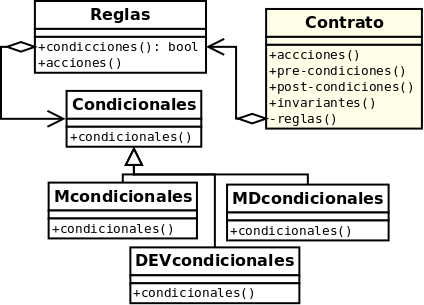
\includegraphics[width=5 in,totalheight=4 in] {Ch9/f2}
 % .: 0x0 pixel, 0dpi, 0.00x0.00 cm, bb=
\end{center}
\caption{Elementos y relaciones relevantes en la creación de los condicionales}

Partiendo de una de las propiedades de las reglas de los contratos sobre la
posibilidad de definir comportamientos a través de parámetros context-aware e
inducidos por reglas donde se designan partes de las acciones del contrato. De
esta manera, las reglas forman parte de un mecanismos de agregación encargado de
la composición de diferentes tipos de condicionales, en los que se encuentran
una familia de condicionales (Condicionales DEVS) conectados a los métodos que
implementan las métricas definidas particularmente para la simulación de
interacciones (sección 4). Las otras dos familias de condicionales representadas
por las clases Mcondicionales y MDcondicionales se comportan de manera similares
teniendo en cuenta el mismo modelo de integración propuesto [10].
A continuación se describen los aspectos principales que se tuvieron en cuenta
en la integración de los anteriores sistemas de coordinación de contratos
sensibles al contexto y extensiones de condicionales para la aplicación de un
nuevo sistema de métricas de interacciones mediante un modelo de simulación
DEVS. 

\subsection{Modelo conceptual de integración}

Para implementar la invocación de métricas mediante métodos correctos,
propusimos  desde la perspectiva del rediseño e implementación computacional, un
modelo de integración de muy bajo costo, sin cambios sustanciales ni en la
arquitectura original  ni en el código de la implementación dentro de la
aplicación modificada en el proceso de inyección de las propiedades de
coordinación de contratos sensibles al contexto [3].


El modelo conceptual de métrica pertenece al Modelo INCAMI (Information Need,
Concept model, Attribute, Metric and Indicador: Información relevante, Modelo
Conceptual, Atributos, Métricas e Indicadores) [12]. INCAMI es un framework
organizacional, orientado a la medición y evaluación que permite economizar
consistentemente, no sólo metadata de métricas e indicadores, sino también
valores mensurables en contextos físicos.


Por medio de un diagrama UML, se representa un modelo general de integración,
teniendo en cuenta experiencias vinculadas al agregado de nuevas componentes en
determinadas implementaciones resueltas para sistemas e-learning similares al
diseño del framework [2]. La integración se produce mediante la conexión de las
reglas, a través de sus condicionales, con una métrica representada con un
método. A su vez,  la métrica es interpretada por un modelo DEVS diseñado para
devolver valores de simulación [13].


En la figura 3 se puede observar lo correspondiente a cada una de las áreas
mencionadas, representadas con colores diferentes. Además, se muestra que la
principal componente para lograr la integración está representada por la
incorporación de una relación de agregación entre la componente Contrato y la
entidad Método. Los condicionales de las reglas de los contratos son invocados
(mediante un método explícito relacionado con la noción de los Condicionales
DEVS, por ejemplo, getForumTheme) por medio de un mecanismo de callback que
permite la correcta invocación de la métrica.
La primera fase de la misma corresponde a la definición y especificación de
requerimientos. Este módulo trata con la definición de la necesidad de
información (es decir, el foco de la evaluación) y el diseño de los
requerimientos no funcionales, que servirán como guías para las actividades
posteriores de medición y evaluación.



\begin{center}
 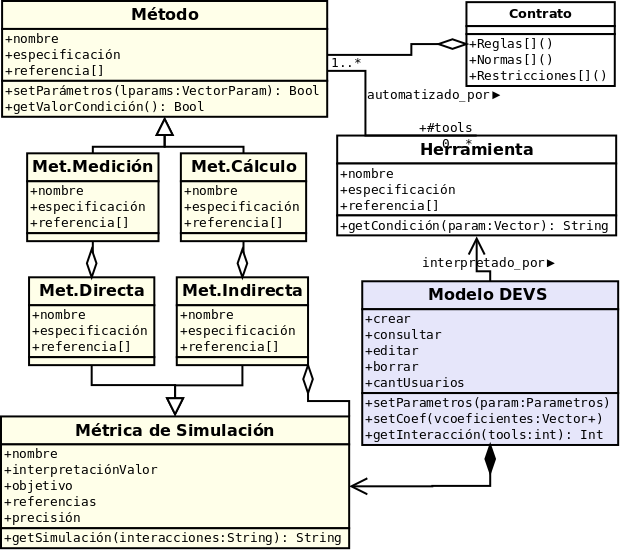
\includegraphics[width=3 in,totalheight=4 in] {Ch9/f3}
 % .: 0x0 pixel, 0dpi, 0.00x0.00 cm, bb=
\end{center}
\caption{Modelo de integración para contractos, métricas y modelo DEVS.}

Tomamos como punto de partida la descripción del Dispositivo Hipermedial
Dinámico [14]. De esta manera se desprende que la información necesaria en
nuestro caso es función de las interacciones de los participantes, las cuales
estarán definidas por: id del participante, rol del mismo, Paquete Hipermedial
(PH) sobre el cual participa, tipo de PH, herramienta sobre la cual realiza la
interacción, tipo de herramienta, servicio con el cual interactúa y el tiempo,
día y hora de la interacción [13].
El principal objetivo de la implementación de la evaluación global permite
mayores niveles de flexibilización para los valores de los indicadores globales
y parciales, a partir de los valores de indicadores elementales utilizando el
modelo de agrupamiento obtenido para efectuar el cálculo. En este proceso,
dichos valores deben ser acordados y consensuados por expertos con experiencia
en el uso de este tipo de sistemas. El seteo de los coeficientes serán
establecido a través de la interface setcoeficient, de la clase Modelo DEVS
(figura 3). En cada caso, el valor resultado brinda una medida sobre el grado de
interactividad de la participación. El responsable de la evaluación pueda dar
valor a los diversos coeficientes subrayando aquel atributo que considere más
importante en el proceso. En cada caso, el valor resultado brinda una medida
sobre el grado de interactividad de la participación. Este valor se obtiene a
través de la interfase getInteracción, que toma como argumento en este caso un
número entero que identifica la herramienta.

Por último mencionamos que la interfase setParametros queda reservada para
posibilitar diferentes relaciones algebraicas dentro de la métrica potenciando
el nivel de expresión de la misma.

La interpretación y manipulación de los resultados de interacciones resueltos en
el Modelo DEVS es manipulado por una herramienta representada por la clase
Herramienta. A su vez la herramienta es la encargada de brindar la información
necesaria sobre los parámetros que necesita la clase Método que es utilizada
como argumento de la función setParámetro. El método getValorCondición
representa los valores de verdad del condicional que formará parte de la regla
explícita representada por el método reglas de la clase Contrato.
Técnicamente la Herramienta es una aplicación que respeta la arquitectura del
framework colaborativo SAKAI [7], utilizando los servicios base para el acceso a
la base de datos. Por otro lado,  permite la aplicación de una función
transferencia que transforma dichos datos teniendo en cuenta un archivo de
parametrización. En nuestros desarrollos se utilizó iBbatis
(http://ibatis.apache.org/) para el acceso a datos y XML DOM
[http://msdn.microsoft.com/en-us/library/ms764730%28VS.85%29.aspx] Parser para
la parametrización de la función transferencia. Los demás componentes
tecnológicos que complementan el desarrollo cumplen los estándares del
framework, en este caso se utilizaron Servlets y Beans teniendo en cuenta el
acceso a los servicios base del framework que permitan el registro de la
aplicación como herramienta.

\subsection {Implementación en un caso de uso}

A continuación se describe un caso de uso para ejemplificar las distintas etapas
que se deben cumplimentar como usuario para la activación de las propiedades que
brindan los Condicionales DEVS dentro de los contratos sensibles al contexto
(sección 2). Además, se brindarán detalles funcionales sobre el uso de la
herramienta Sakai que implementa la conexión entre los métodos de la métrica y
el modelo de simulación DEVS, manteniendo la perspectiva de un usuario final.
Se comienza con el diseño de las reglas de los contratos y sus correspondientes
condicionales DEVS. Para esta etapa tomaremos como referencia el esquema para el
diseño de contrato propuesto en UWATc en la última etapa del diseño de procesos
e-learning Web [10].

\subsubsection{Representación de los Condicionales DEVS a través de UWATc}

En UWATc se brinda un diagrama de representación de contrato, donde se describen
todos los datos que lo instancian. Cada tipo de dato y valor, pertenece a un
elemento del metamodelo de la figura 1.

Teniendo en cuenta el diagrama siguiente, en primer lugar (item 1) se
identifican los objetos participantes en el contrato; en dicho ejemplo
DiscussionAction y UserAction hacen referencia a dos clases reales perteneciente
a la implementación de la herramienta Foro y Usuarios de una aplicación,
respectivamente. Luego, se identifican los nombres de los parámetros
context-aware significativos para el contrato, alineados en la misma columna del
objeto que lo comparte (item 2). En Servicios (item 2) deben ser representados
los métodos del objeto, que al ser ejecutados, provocan la intervención del
contrato. Para este ejemplo initState y getIdentifier son ejecutados cuando un
usuario ingresa a la herramienta Foro y las posteriores funcionalidades
(servicios) disponibles dependen de la ejecución del contrato Edición. Las
siguientes filas (item 2) se refieren a las pre y post-condiciones que se deben
cumplir en la ejecución del contrato.


Por último se explicitan las reglas de coordinación (item 3). Siguiendo con el
ejemplo, en la parte del condicional u.contexto =' l1; p1; docente; r1; c1; IT1;
IPH1'  verifica si el contexto del usuario u está compuesto por la locación l1,
tienen el perfil p1, es un docente, cumple el rol r1 y pertenece a la categoría
c1 (este tipo de representación de contexto se encuentra desarrollado en [2]).
Además, los últimos dos valores IT1 y IPH1, representan el nivel de
interacciones que un determinado usuario y de una herramienta particular,
respectivamente. A diferencia de los otros valores, IT1 y IPH1 serán comparados
con la resultante de la aplicación de una métrica de interacción a través de un
elemento externo con interfaz para comunicarse a través de los Condicionales
DEVS.

\begin{center}
 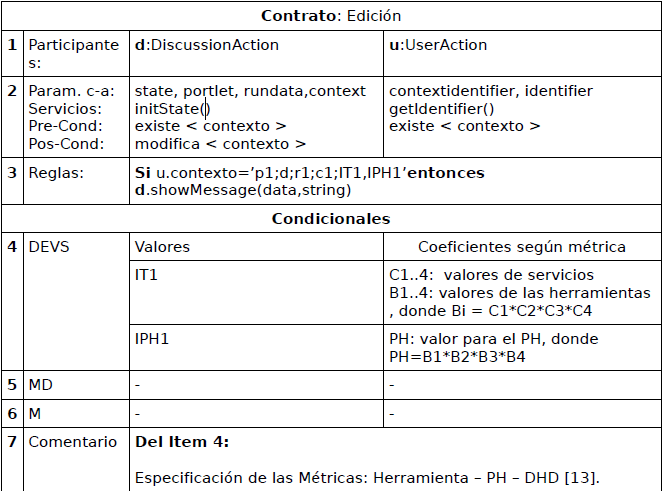
\includegraphics[width=5 in,totalheight=4 in] {Ch9/f4}
 % .: 0x0 pixel, 0dpi, 0.00x0.00 cm, bb=
\end{center}
\caption{Modelo de integración para contractos, métricas y modelo DEVS.}

En el item 4 se describe la forma de representar en el diagrama que dichos
valores pertenecen al tipo de Condicional DEVS y la definición de los
coeficientes que formarán parte de la métrica y serán alcanzado por los valores
de los parámetros de las interfaces de los métodos que la representan.
En cuanto a la acción de la regla de coordinación, continuando con el mismo
ejemplo, en el item 3 se induce  la ejecución del método showMessage del objeto
d (DiscussionAction). El final del diagrama está dedicado a comentarios
generales; cada comentario debe ir acompañado con el número al que hace
referencia.


De esta manera, a través de la extensión del diagrama de contrato de la etapa 4
en el proceso de diseño de los Pe-lrn [10] se logra describir los principales
componentes que se tienen en cuenta en el diseño e implementación de los
Condicionales DEVS  para los casos de uso similares al presentado.

\subsubsection{Ejemplo de ejecución de la métrica en PowerDEVS}


Atendiendo a lo expuesto, seguidamente se implementan lo explicado en el entorno
PowerDEVS [15] teniendo en cuenta el mismo caso de uso introducido en esta
sección. En la figura 3, la clase Modelo DEVS contiene las interfaces que son
implementadas a través de la herramienta PowerDEVS para la interpretación de las
métricas presentes en el comentario del diagrama de contrato.


Cada métrica directa tiene asociado un método de medición claramente
especificado. Las colecciones de datos son capturados desde la bases de datos
(en este caso MySQL). Luego los datos son formateados para posibilitar su
lectura desde el entorno.


En la figura 4 se muestran, a manera de ejemplo, los resultados obtenidos de
Nivel de Interactividad para cada participación a través del tiempo, en los
meses de Noviembre-Diciembre para un curso seleccionado en el 2009, del Campus
Virtual de la Universidad Nacional de Rosario
(http://www.campusvirtualunr.edu.ar).

\begin{center}
 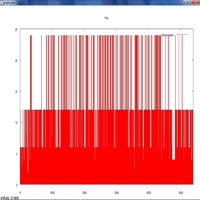
\includegraphics[width=5 in,totalheight=4 in] {Ch9/f5.png}
 % .: 0x0 pixel, 0dpi, 0.00x0.00 cm, bb=
 % Es el de las gráficas
\end{center}
\caption{Resultados obtenidos en el entorno PowerDEVS.}


Cabe mencionar que los resultados obtenidos son los globales del DHD, pero que
sin embargo se disponen a su vez, los valores parciales tanto a nivel Paquete
Hipermedial, como a nivel Herramienta individual, (por cuestiones de espacio
nomostramos aquí dichos gráficos). Los mismos se exportan a un archivo que 
relaciona el número de participación, con su nivel de interactividad.


El resultado de este análisis es considerado una información de contexto,
resignificando una característica del comportamiento de los participantes y
atendiendo a la posibilidad de usar la información de interactividad como
parámetro context-aware de los contratos [3]. Podremos entonces, establecer un
lazo de retroalimentación entre las prácticas efectuadas en los entornos
colaborativos, informadas en el Registro de Actividad y las acciones que
devengan de los contratos.

\subsection{Conclusiones}

En este trabajo se fundamentó la posibilidad de extender las propiedades
expresivas de las reglas de coordinación de contratos de los DHD a partir de los
resultados de un mecanismo externo. La propuesta de integración expuesta sigue
respetando las líneas de diseño e implementación establecidas por el modelo de
los DHD. 
Ahora se tiene un nuevo mecanismo para la escritura de las reglas de los
contratos que permitirá ahorrar esfuerzo en el diseño de los condicionales que
verifiquen información de contexto parametrizado. Además, se evita la necesidad
de tener conocimiento sobre las leyes (diseño) de las métricas y su
implementación, con sólo tener información sobre la definición de los
coeficientes que participan en la métrica. 


\section{SEPI: una herramienta para el Seguimiento y Evaluación de
Procesos Interactivos del DHD}


\subsection{Introducción}

Las actuales Tecnologías de la Información y Comunicación (TIC) han posibilitado
la construcción de una nueva realidad físico-virtual donde los sujetos pueden
ser partícipes de diversas redes sociotécnicas. Estas redes están conformadas
por una multiplicidad de componentes y relaciones, que se configuran y
reconfiguran por las diversas interacciones mediatizadas, en función de una gran
diversidad de requerimientos.


La necesidad de evaluar y propiciar una mejor calidad de los procesos
interactivos, cuyos propósitos se centren en investigar, educar y/o producir a
partir de la participación responsable en contextos físicos-virtuales, adquiere
especial relevancia para la construcción conjunta e inclusiva de la denominada
“Sociedad de la Información y del Conocimiento”. En atención a esta necesidad
insoslayable, el presente trabajo describe tecnológicamente el primer prototipo
de una herramienta integrada denominada “SEPI-DHD” que colabora en el
Seguimiento y Evaluación analítica de los mencionados procesos de interacción
mediatizados por un Dispositivo Hipermedial Dinámico (DHD) retroalimentando
información de contexto de los participantes.


Se conceptualiza como DHD a una red sociotécnica [1] conformada por la
conjunción de tecnologías y aspectos sociales que posibilita a los sujetos
realizar con el otro, acciones en interacción responsable para investigar,
aprender, dialogar, confrontar, componer, evaluar, diseminar bajo la modalidad
de taller físico-virtual, utilizando la potencialidad comunicacional,
transformadora y abierta de lo hipermedial [2], reguladas según el caso por una
“coordinación de contratos” [3].


De esta manera, el DHD se constituye como una entidad compleja [4] compuesta por
la integración de dos dimensiones indisociables: una técnica (o conjunto de
técnicas constructivas que comportan una materialidad y una configuración
particular) y una social dada por las relaciones intersubjetivas y la situación
en la que se inscriben.


La necesidad de SEPI-DHD, se fundamenta en el marco de dos requerimientos de I+D
relacionados: el primero está referido a la importancia de efectuar análisis
evaluativos de los desarrollos e implementaciones llevados adelante en el
entorno colaborativo de I+D+T del Programa “Dispositivos Hipermediales
Dinámicos” [5]. El segundo requerimiento, se encuentra en una fase experimental
e investigativa y está relacionado con la implementación de un original
desarrollo de pieza de software denominada “contrato” que debe ser ubicada
reflexivamente en el sistema por los usuarios calificados para diseñar e
implementar el espacio de formación, investigación y/o transferencia con la
finalidad de potenciar el aspecto dinámico de los procesos de interacción
responsable del DHD [6].


En referencia a dichos requerimientos, adoptó la utilización del formalismo DEVS
(Discrete EVents dynamic Systems) [7] que propone una teoría de modelado de
eventos discretos en sistemas a tiempo continuo, permitiendo a su vez, una
descripción modular de los fenómenos y el abordaje de la complejidad usando una
aproximación jerárquica. En la implementación de dicho formalismo se integran
las métricas de ponderación siguiendo las recomendaciones del framework INCAMI
[8].

A su vez, tecnológicamente el entorno colaborativo de prueba está provisto por
un agregado de una pieza de software para la inyección de propiedades de
coordinación de contratos sensibles al contexto [9]. Esta propiedad se logra a
través de la implementación de contratos [10] con mecanismos de coordinación y
componentes de sistemas Context-Aware. La utilización de reglas es esencial para
la implementación de las acciones de los contratos estando compuestas por los
condicionales, en donde se centra parte de la lógica de adaptación que requiere
el DHD. Algunos condicionales implementados requieren de mecanismos externos que
colaboren en la composición de sus valores de verdad que son ponderados a partir
de simulaciones por medio del modelo DEVS [11]. La herramienta SEPI-DHD de
código abierto funcionalmente logra la integración tecnológica de los
Condicionales DEVS, pertenecientes a los contratos con el módulo de ejecución
del modelo DEVS [12].

En la siguiente sección describiremos los elementos tecnológicos del DHD en
relación directa con los Condicionales DEVS.  Luego, en la sección 3
presentaremos el modelo de integración adoptado para la implementación de la
herramienta. En la sección 4 abordaremos algunas de las características,
funcionalidades y un caso de uso concreto para arribar finalmente a breves
conclusiones y prospectiva del desarrollo.


\subsection{Elementos para la integración}

En esta sección describiremos aspectos tecnológicos y componentes del DHD que la
herramienta SEPI toma en cuenta para la conexión entre los Condicionales DEVS y
las métricas de interacción DEVS. 

Sintéticamente, los Condicionales DEVS son condicionales simples que pertenecen
a un conjunto de reglas que definen acciones dentro de componentes
computacionales contratos. Los contratos, definidos por  Meyer [10], se basan en
la metáfora de que un elemento de un sistema de software colabora con otro,
manteniendo obligaciones y beneficios mutuos. En este caso, los contratos son
objetos de primera clase dentro de la original propuesta tecnológica del DHD [6]
donde se le agregan propiedades de sensibilidad al contexto y dinamismo. 
Dado que la evaluación sobre los valores de verdad de los Condicionales DEVS se
referencian en resultados obtenidos al ejecutarse un simulador de un modelo de
eventos discretos que representa una métrica cuali-cuantitativa [12], podemos
afirmar que estos condicionales promueven nuevas propiedades de adaptación del
DHD posibilitando que las reglas de los contratos tengan mayor grado de
expresión. 

En la siguiente Figura 1, se muestra cuales son los elementos que se deben tener
en cuenta para implementar los valores calculados que deben contrastarse con
valores testigos para formar los condicionales de las proposiciones lógicas de
las reglas.  Las  relaciones entre las componentes influyen en elementos
conceptuales que determinarán algunas de las características funcionales de los
requerimientos del DHD [9] relacionados a los requisitos de comportamiento y
configuración.

La herramienta cuenta con tres tipos de servicios que derivan del núcleo base
del framework del DHD, uno de ellos (S.Conexión) encargado de establecer la
conexión para incorporar valores calculados dentro de los Condicionales DEVS.
Otro tipo de servicio (S.Ejecución) implementa las secuencias de ejecuciones del
modelo DEVS  que obtiene los resultados de las interacciones. Algunos de estos
pasos serán descriptos en la sección 4 y forman parte de los requisitos que se
deben cumplir para ejecutar la simulación implementada en el módulo DEVS
(ModDEVS), que en este caso se ajusta a las interfaces que provee PowerDEVS
[13].

El último servicio que extiende los servicios base (S.Configuración) se encarga
de implementar todas las cuestiones de configuración de la métrica que provienen
de la interfaz de usuario. En este caso se provee al usuario de un prototipo de
interfaz que permite establecer las ponderaciones de los coeficientes de la
métrica de interacción representada en DEVS, para que luego se puedan
transformar en los parámetros necesarios al invocar el método de configuración
de S.Configuración. El componente Configuración refiere a la relación entre el
servicio de interfaz (S.Conf) y los elementos utilizados para implementar la
interfaz del usuario de la herramienta, en este caso representada con la clase
UIUsuario.


\begin{center}
 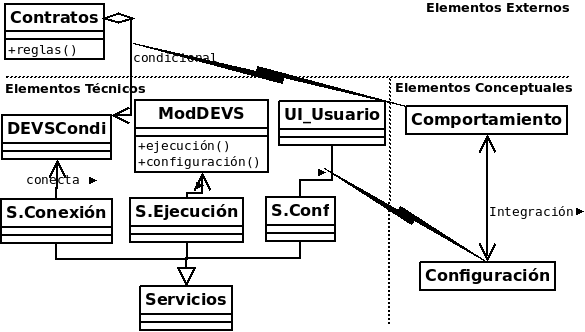
\includegraphics[width=5 in,totalheight=4 in] {Ch9/f11}
 % .: 0x0 pixel, 0dpi, 0.00x0.00 cm, bb=
\end{center}
\caption{Modelo de elementos y relaciones de los DEVS condicionales.}
                 

De esta manera queda establecida una relación conceptual entre los servicios
(Servicios) y los contratos que definen el comportamiento adaptativo de algunas
de las acciones del DHD. Esta última relación fue representada en la Figura 1
mediante la relación de agregación entre el contrato (Contrato) y el Condicional
DEVS (DEVSCond),  determinada por la relación conceptual Comportamiento. 
Las interfaces de los métodos las abordaremos seguidamente como parte de la
herramienta que implementa el modelo de integración. De esta manera queda
establecida una nueva relación conceptual, llamada relación de Integración, a
partir de las componentes conceptuales Comportamiento y Configuración.  


Cabe destacar que los elementos conceptuales representados en la figura forman
parte de los requerimientos de adaptabilidad que debe cumplir el DHD [6]. A su
vez, los elementos técnicos pertenecen al diseño propuesto para el modelo de
integración que se implementa a través de la herramienta. Las funcionalidades
que interpretan el servicio de ejecución las describiremos en la sección 4.


\subsection{Modelo conceptual de integración}

En esta sección representaremos un modelo general de integración teniendo en
cuenta experiencias vinculadas al agregado de nuevas componentes en determinadas
implementaciones resueltas para entornos colaborativos similares al diseño del
framework [6]. En este caso, el modelo determina los componentes, sub-sistemas y
relaciones sobre la herramienta de integración encargada de articular los
resultados de la simulación del modelo DEVS para insertarlo en los contratos. 


En la siguiente Figura 2 observamos una primera conexión entre los servicios de
la herramienta, que fueron introducidos en la sección anterior, con el modelo de
simulación DEVS. Para este caso contamos con los métodos del módulo Integrador, 
representado por una clase UML [14] que implementan las secuencias de
ejecuciones que se deben respetar para que el intérprete DEVS (en este caso
PoweDEVS [13])  tome los valores de entrada adecuados (método getInputDEVS) que
son procesados por medio de una función transferencia parametrizada (método
setTransferencia) a partir de un archivo de configuración XML. Luego se toman
los valores de salida (método getOutputDEVS) para su posterior procesamiento.
Todos los datos de entradas son extraídos de la base de datos perteneciente al
entorno colaborativo utilizado, a través de métodos privado getDB. Los
parámetros que implican la ejecución del simulador DEVS deben ser alcanzados por
las interfaces representadas en la clase Integrador. 


\begin{center}
 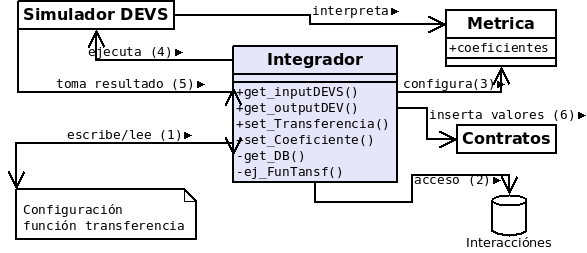
\includegraphics[width=5 in,totalheight=4 in] {Ch9/f12}
 % .: 0x0 pixel, 0dpi, 0.00x0.00 cm, bb=
\end{center}
\caption{Modelo de integración para contratos, métricas y modelo DEVS.}

Las cuestiones de parametrización y representación de los valores, pre y
pos-condiciones que se encuadren en un nivel superior para lograr una mejor
interpretación y manejo por parte de los usuarios se guardan en el archivo de
configuración e interviene el servicio S.Configuración  mencionado en la
sección 2.


Si bien, en este caso, el diseño de integración propuesto se basa en la
descripción   de componentes de software de la herramienta de integración aquí
propuesta, es necesario tener en cuenta otros elementos que en este diseño no se
muestran. En otro trabajo [15] hemos desarrollado lo correspondiente a cada una
de las áreas mencionadas con un nivel más profundo de detalle. Además, se
muestra que la principal componente para lograr la integración está representada
por la incorporación de una relación de agregación entre una componente Contrato
y una entidad Método que se corresponde con la arquitectura que propone INCAMI
[8] para la construcción de métricas.


En términos generales, la SEPI-DHD es una aplicación que respeta la arquitectura
del framework, utilizando los servicios base para el acceso a la base de datos.
Por otro lado, permite la aplicación de una función transferencia que transforma
dichos datos teniendo en cuenta un archivo de parametrización. Los diversos
componentes tecnológicos que complementan el desarrollo cumplen los estándares
del framework, en este caso utilizamos Servlets y Beans teniendo en cuenta el
acceso a los servicios base del framework que permitan el registro de la
aplicación como herramienta.


\subsection{Implementación en un caso de uso}

A continuación desarrollaremos un caso de uso brindando detalles funcionales
sobre la herramienta desde la perspectiva de un usuario final. Dicho camino se
divide en seis pasos metodológicos coincidentes con las relaciones descriptas
en la Figura 2.

\paragraph{Paso 1: Escritura y lectura del XML}

La herramienta contiene una interfaz apropiada para la representación de los
coeficientes que componen la métrica, permitiendo de esta manera que el usuario
controle las ponderaciones que reflejan propiedades cuali-cuantitativas sobre
las interacciones de los participantes. Se presentan los pesos necesarios (Rol,
Tipo de Paquete Hipermedial, Tipo de Herramienta, Tipo de Servicio) con un valor
por defecto igual a 1 (para los valores nulos el valor por defecto es cero). A
su vez se da la posibilidad de modificar esos valores a través de la opción
Modificar Ponderación, seleccionando el coeficiente y el subtipo de coeficiente.
Luego se crea automáticamente un archivo XML donde se detallan todos los valores
necesarios para que la función transferencia procese las tablas y valores de sus
campos que sirvan como entradas al simulador DEVS. La siguiente tabla describe
el significado de las marcas (“tags”)  donde se brindan los detalles concretos
para los parámetros de las interfases de cada subsistema de la sección 3.


\begin{center}
 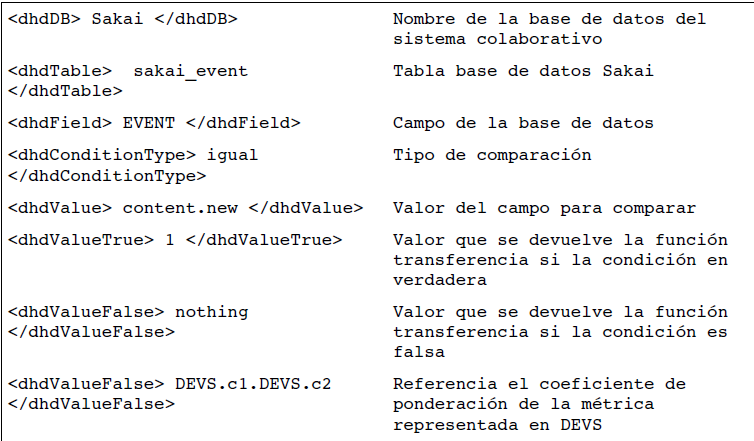
\includegraphics[width=5 in,totalheight=4 in] {Ch9/f13}
 % .: 0x0 pixel, 0dpi, 0.00x0.00 cm, bb=
\end{center}
\caption{Modelo de integración para contratos, métricas y modelo DEVS.}



\paragraph{Paso 2: Acceso a la base de datos}


Si bien este paso es transparente para el usuario final los diseñadores e
implementadores deben cumplir con ciertos requisitos que se ajustan a las
necesidades del modelo de integración aquí propuesto. En este sentido se
establecen diferentes tipos de conexiones entre subsistemas a través de mensajes
y secuenciación  de ejecución de tareas (ej, relación toma resultado (5),
sección 3). Por otro lado, es necesario implementar acciones de penetración
entre sistemas que deben respetar una infraestructura tecnológica y de diseño,
este es el caso de la vinculación que se propone en el modelo de integración
entre el módulo Integrador y la base de datos que contiene las interacciones
(relación acceso (2), sección 3).


En este caso, proponemos un modelo de acceso a base de datos a través de iBATIS 
teniendo en cuenta que la capa de abstracción será la interfaz con la capa de la
lógica de la función transferencia, haciendo las veces de “facade” entre
laaplicación y la persistencia. Teniendo en cuenta el patrón Data Access Object
(DAO), nuestra implementación  utilizó  del framework DAO (ibatis-dao.jar). La
capa de Framework de Persistencia será la interfaz con el gestor de Base de
Datos ocupándose de la gestión de los datos mediante el framework
SQL-MAP (ibatis-sqlmap.jar).

En la siguiente Figura 3, mostraremos un ejemplo de  las clases y relaciones que
implementa el acceso a la tabla sakaiEvent de la base de datos Sakai.


\begin{center}
 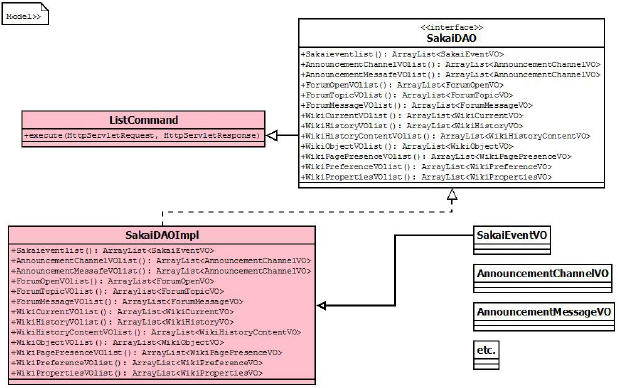
\includegraphics[width=5 in,totalheight=4 in] {Ch9/f14}
 % .: 0x0 pixel, 0dpi, 0.00x0.00 cm, bb=
\end{center}
\caption{Estructura para el acceso a la Base de Datos.}


\paragraph{Paso 3: Configuración de coeficientes de la métrica}


A partir del acceso a la base de datos, la aplicación genera un archivo
input.csv en el cual se guardan los vectores (de ocho componentes) [12] que
serán los datos de entrada del entorno utilizado para correr el modelo DEVS que
integra las métricas (relación acceso (3), sección 3). Cada métrica directa
tiene asociado un método de medición claramente especificado.


\paragraph{Paso 4: Ejecución de la simulación}

Una vez generados los valores de entrada correctos, estos serán utilizados en la
simulación. Se ejecutará el modelo DEVS general como un módulo model.exe que
posee dos parámetros, el archivo de entrada antes generado: input.csv, y el
número de eventos totales (relación acceso (4), sección 3). Luego de la
ejecución se genera el archivo output.csv el cual contiene los valores de
niveles de interactividad para cada participación.

\paragraph{Paso 5: Lectura de resultados}


A continuación, la Figura 4 muestra gráficamente a modo de ejemplo, los
resultados obtenidos de Nivel de Interactividad para cada participación a través
del tiempo en el entorno colaborativo de investigación del Programa DHD, antes
mencionado. La interfase posibilita diversos filtrados y colorea los niveles de
interactividad según los requerimientos del usuario (relación acceso (5),
sección 3).


\begin{center}
 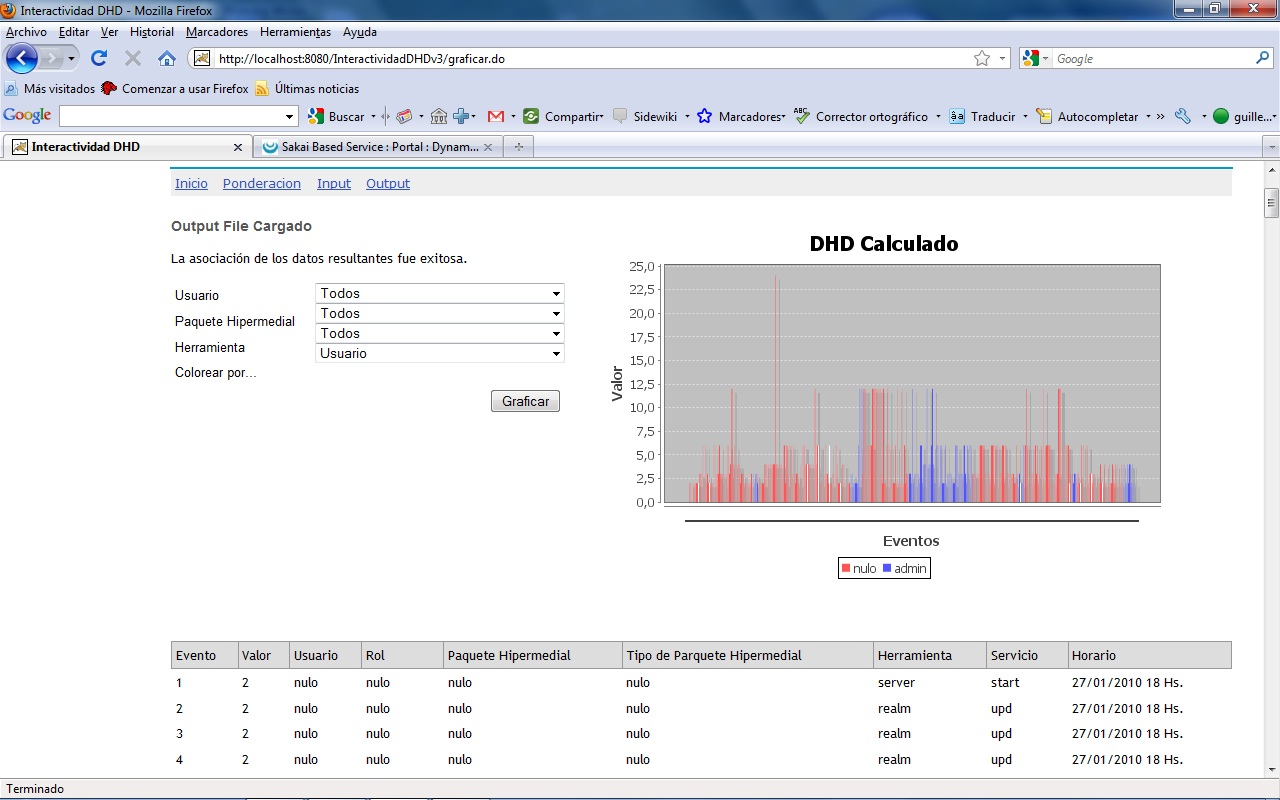
\includegraphics[width=5 in,totalheight=4 in] {Ch9/f15}
 % .: 0x0 pixel, 0dpi, 0.00x0.00 cm, bb=
\end{center}
\caption{Estructura para el acceso a la Base de Datos.}

\paragraph{Paso 6: Insertar valores en los contratos}


El resultado de este análisis es considerado una información de contexto,
resignificando una característica del comportamiento de los participantes y
atendiendo a la posibilidad de usar la información de los niveles de
interactividad como parámetro context-aware de los contratos (relación acceso
(6), sección 3).

\subsection{Conclusiones}


En este trabajo hemos presentado la herramienta integrada SEPI para el
seguimiento y evaluación de procesos de interacción del DHD adaptado al entorno
colaborativo SAKAI. A su vez, se extendieron las propiedades expresivas de las
reglas de coordinación de contratos del DHD a partir de los resultados de un
mecanismo externo. De esta manera, es posible establecer un lazo de
retroalimentación entre las acciones efectuadas en los entornos colaborativos y
las que devengan de los contratos.


Además de las cualidades funcionales logradas, la herramienta SEPI concreta la
integración de los subsistemas por medio de mensajes, ejecución de tareas y
penetración, atendiendo a las líneas de diseño e implementación establecidas
dentro del marco teórico-metodológico del DHD.
La prospectiva actual se centra en la optimización de la herramienta, su prueba
en diversos escenarios de uso y la puesta a disposición de la misma en los foros
de discusión con la documentación correspondiente.
